\documentclass{article}
\usepackage[utf8]{inputenc}

\title{London Calling}
\author{Artur Cassimiro Alves}
\date{April 2019}

\usepackage{natbib}
\usepackage{graphicx}

\begin{document}

\maketitle

\section{Introdução}
London Calling é o terceiro álbum da banda inglesa The Clash lançado em dezembro de 1979. O álbum mistura influências de diversos gêneros musicais como o reggae, o blues e o rock para criar um som punk único.
\cite{wikipediaLondonCalling}

\begin{figure}[h!]
\centering
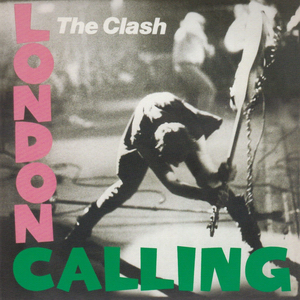
\includegraphics[scale=1.0]{LondonCalling}
\caption{Capa original do álbum}
\label{fig:London Calling}
\end{figure}

\section{Pontos Positivos}
O álbum possui sons extremamente variados e letras surpreendentemente boas, coloridas com a contra-cultura e angústia do movimento punk do Reino Unido.

\section{Pontos Negativos}
O álbum é bem longo e se seus gostos não se alinhem com ele você pode acabar não gostando. (sei lá)

\bibliographystyle{plain}
\bibliography{references}
\end{document}
